%!TEX root = practicum3.tex
To find the intersected edges and compute the intersection points we have used the method \t{find_intersected_edges}, see \autoref{lst:c:find_intersected_edges}. This method calls the method \t{line_segments_intersect} (\autoref{lst:b:intersectLineSegments}) on the edge defined by the points \t{p0} and \t{p1} and the edges of the triangulation. If an intersection is found it adds the indices of the intersected edge in the global list \t{intersected_line_segments} and appends the intersection point to \t{intersection_points}. The intersected edges of the triangulation and the intersection points are presented in \autoref{tab:c:intersectedEdges1}.

\lstinputlisting[float, firstline=194, lastline=211, label={lst:c:find_intersected_edges}, caption={The method \t{find_intersected_edges()}.}]{../assignment3C.py}

To visualize the results we have added the code in \autoref{lst:c:display_1}, the resulting visualization is shown in \autoref{subfig:c:result1}.

\lstinputlisting[float, firstline=115, lastline=130, label={lst:c:display_1}, caption={Part of the method \t{display()} that visualizes the intersected edges and the intersections.}]{../assignment3C.py}

\begin{figure}
	\centering
	\begin{subfigure}[b]{0.45\textwidth}
		\centering
		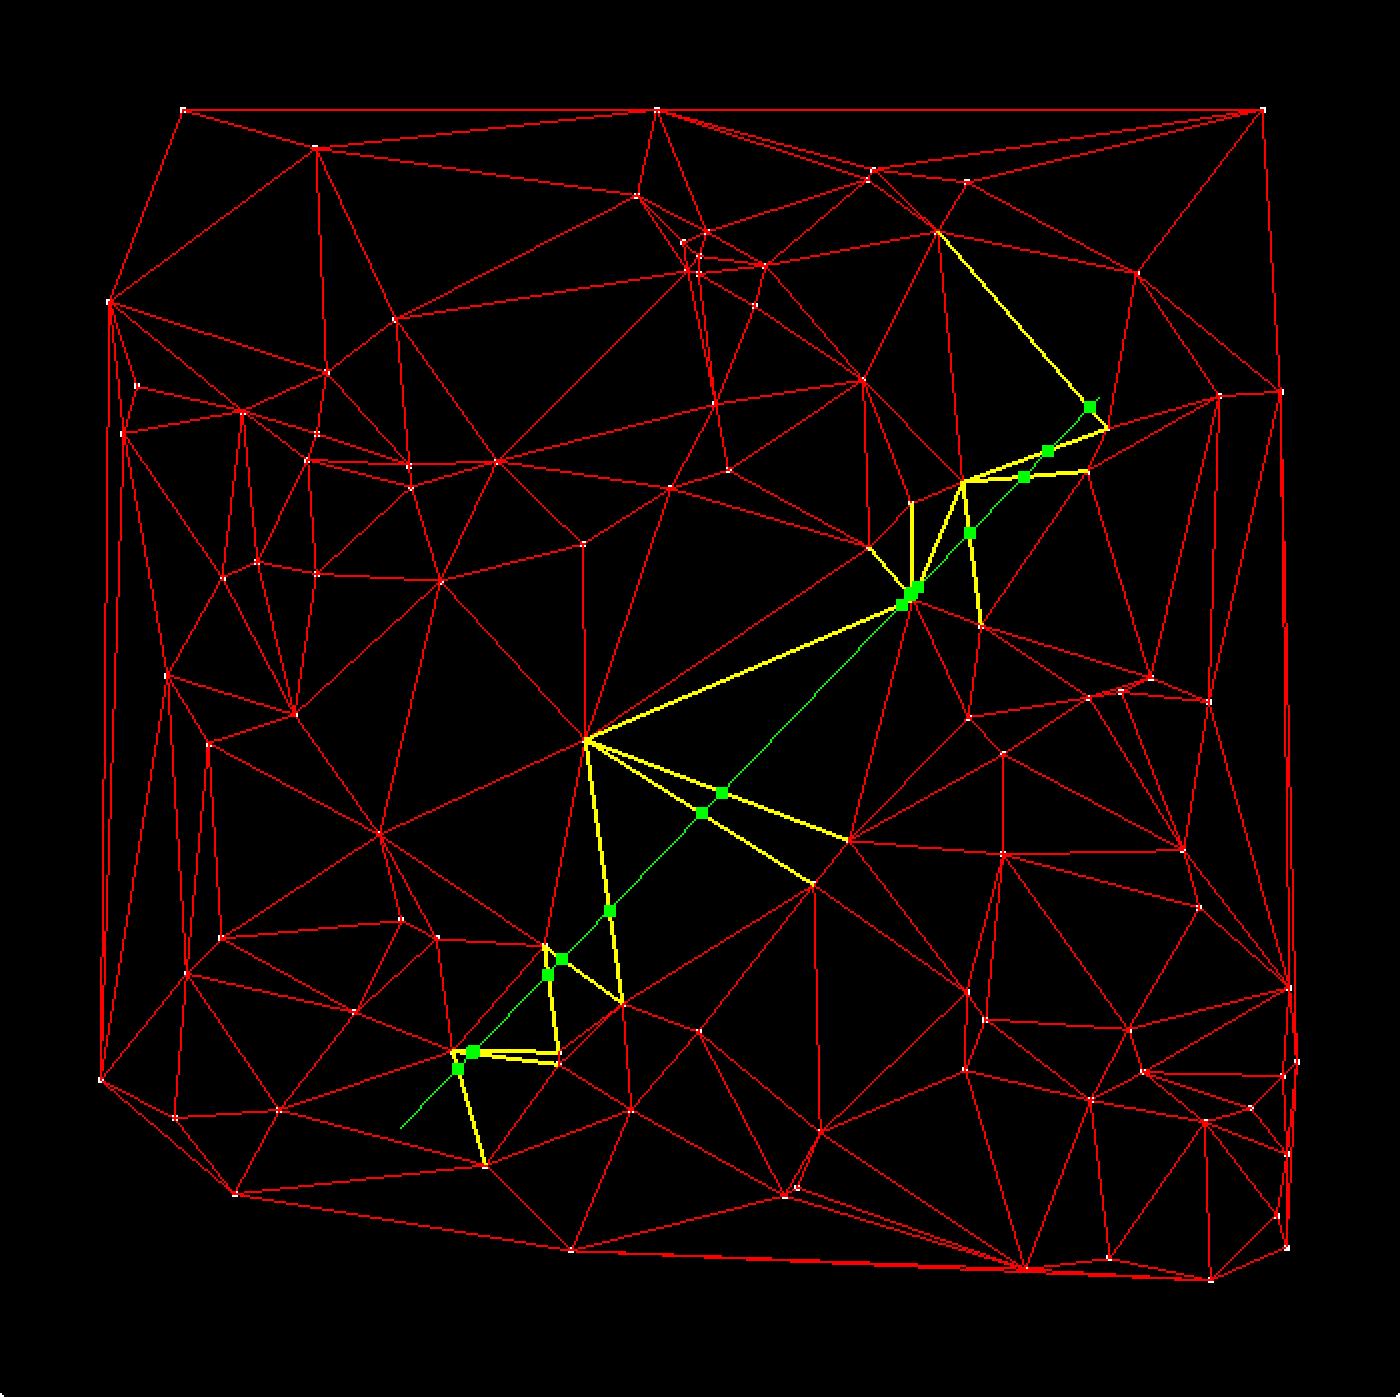
\includegraphics[width=0.9\textwidth]{./img/c_result1}
		\caption{\t{find_intersected_edges}}
		\label{subfig:c:result1}
	\end{subfigure}
	\begin{subfigure}[b]{0.45\textwidth}
		\centering
		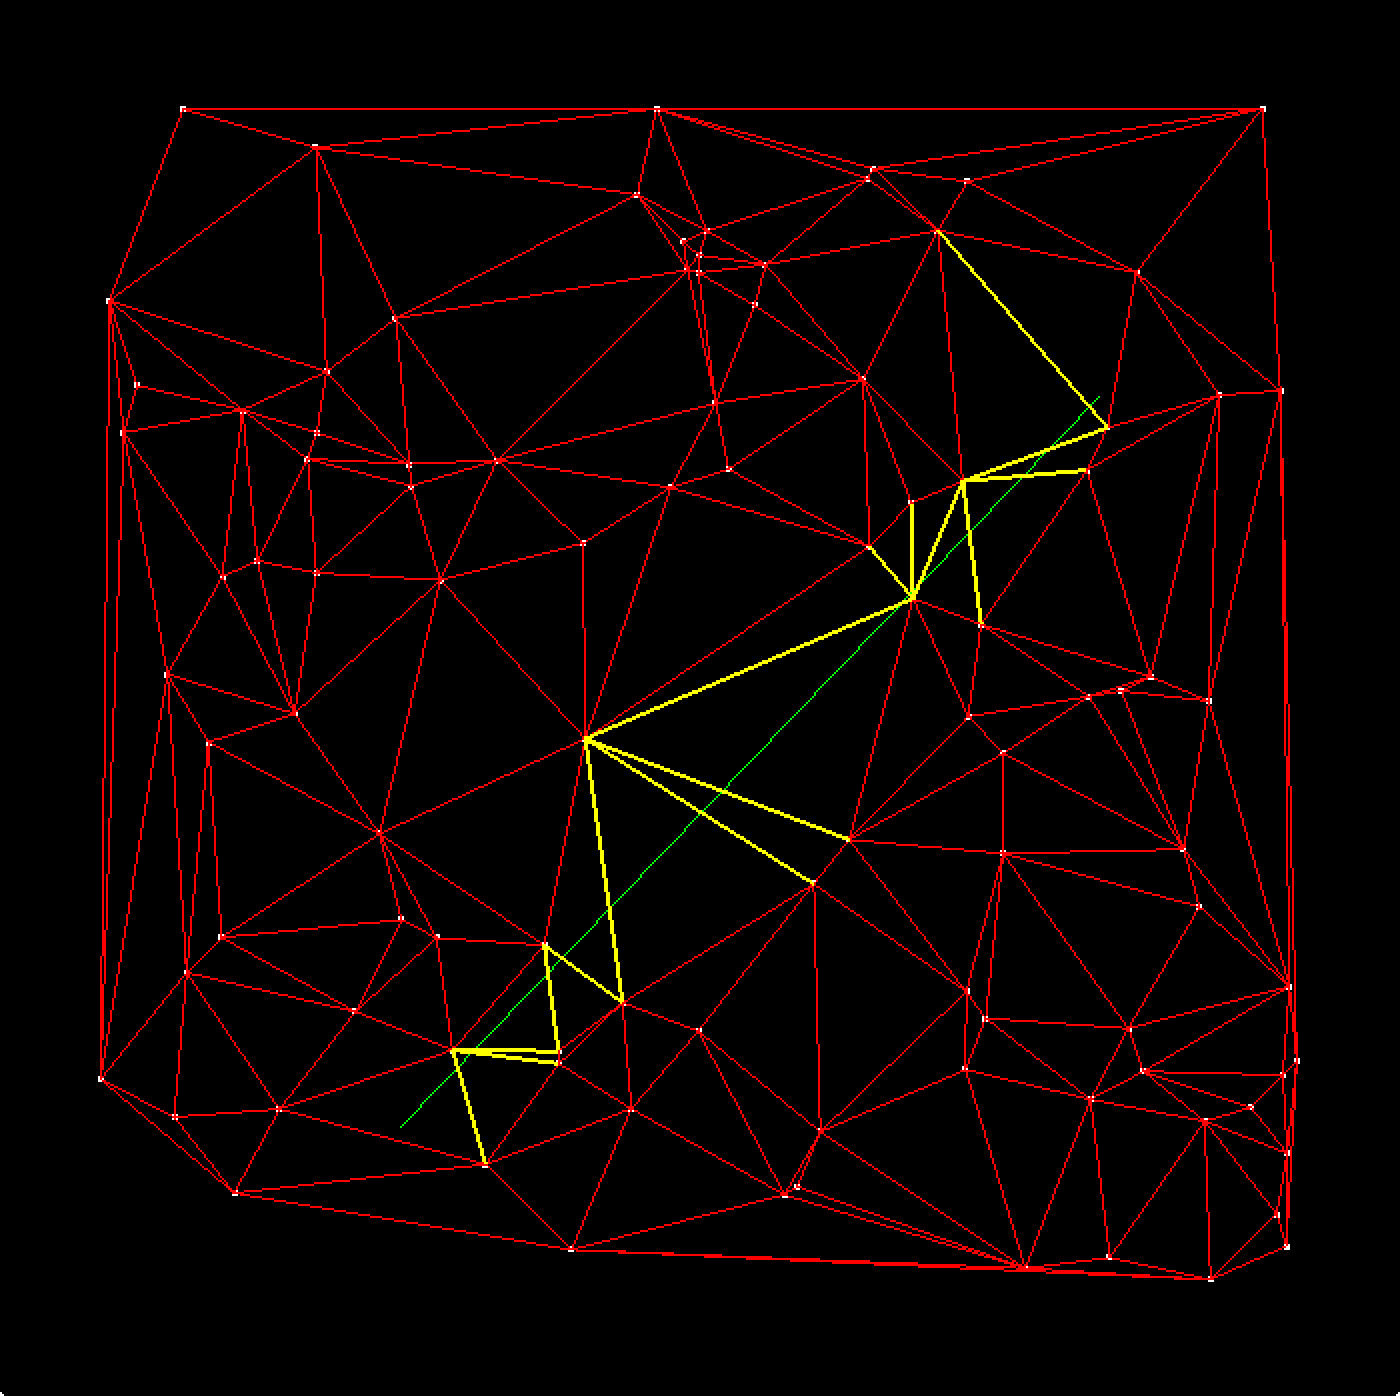
\includegraphics[width=0.9\textwidth]{./img/c_result2}
		\caption{\t{find_edges_on_path}}
		\label{subfig:c:result2}
	\end{subfigure}	
	\caption{The visualization of the intersection of the line segment $s$ with the edges of the triangulation $dt$. Each intersected edge is shown in yellow, and in \autoref{subfig:c:result1} the intersections are represented by green dots.}
	\label{fig:c:result}
\end{figure}

\begin{table}
	\centering
	\footnotesize{
		\begin{tabular}{ll|ll}
		edge & intersection & edge & intersection\\
		\hline
		(\num{226.33195013}, \num{527.007719279}) - (\num{242.796962849}, \num{584.179466813})	&	(\num{228.867696999}, \num{535.812636852})	&	 (\num{456.54758505}, \num{301.329564578}) - (\num{292.651351959}, \num{371.369188947})	&	(\num{450.717707067}, \num{303.820912038})	\\
		(\num{226.33195013}, \num{527.007719279}) - (\num{279.526723944}, \num{533.851551524})	&	(\num{236.087462036}, \num{528.262825414})	&	 (\num{434.746175446}, \num{275.228689898}) - (\num{456.54758505}, \num{301.329564578})	&	(\num{454.940291133}, \num{299.405295558})	\\ 
		(\num{226.33195013}, \num{527.007719279}) - (\num{279.230162351}, \num{527.629726937})	&	(\num{237.165877611}, \num{527.135110841})	&	 (\num{543.382588894}, \num{237.142130429}) - (\num{481.36728233}, \num{242.669629937})	&	(\num{511.78866886}, \num{239.958134849})	\\ 
		(\num{272.14012592}, \num{474.6185968}) - (\num{279.230162351}, \num{527.629726937})	&	(\num{274.010859273}, \num{488.60578716})	&	 (\num{481.36728233}, \num{242.669629937}) - (\num{490.590138248}, \num{314.176426186})	&	(\num{484.674568747}, \num{268.311736682})	\\ 
		(\num{272.14012592}, \num{474.6185968}) - (\num{311.312430627}, \num{503.369689707})	&	(\num{281.098731465}, \num{481.193897954})	&	 (\num{481.36728233}, \num{242.669629937}) - (\num{456.54758505}, \num{301.329564578})	&	(\num{459.283383215}, \num{294.863662123})	\\ 
		(\num{292.651351959}, \num{371.369188947}) - (\num{406.885957326}, \num{443.993258738})	&	(\num{350.781795159}, \num{408.325322776})	&	 (\num{455.757245676}, \num{253.484433518}) - (\num{456.54758505}, \num{301.329564578})	&	(\num{456.489045688}, \num{297.785740795})	\\ 
		(\num{292.651351959}, \num{371.369188947}) - (\num{311.312430627}, \num{503.369689707})	&	(\num{304.689843297}, \num{456.524335295})	&	 (\num{553.745608126}, \num{215.87226731}) - (\num{481.36728233}, \num{242.669629937})	&	(\num{524.448996513}, \num{226.719049361})	\\ 
		(\num{292.651351959}, \num{371.369188947}) - (\num{424.577450772}, \num{421.869738174})	&	(\num{361.075143445}, \num{397.561421426})	&	 (\num{468.981532514}, \num{117.202657047}) - (\num{553.745608126}, \num{215.87226731})	&	(\num{544.790307044}, \num{205.447850348})	\\	 	
		\end{tabular}
	}
	\caption{The edges that were intersected by the line segment between \t{p0} and \t{p1} and the point where the line segment intersected the edge. A point \vec{P} defined by its $x$ and $y$ coordinate is represented as $(x, y)$. A line segment between the points \vec{P_1} and \vec{P_2} is represented as (\vec{P_1}, \vec{P_2}). The first two columns contain the first eight intersected line segments in the order that they were found, the last two columns contain the last eight intersected line segments, once again in the order that they were found.}
	\label{tab:c:intersectedEdges1}
\end{table}

~\\

\noindent To find all consecutive intersection points we use the method \t{find_edges_on_path}, presented in \autoref{lst:c:find_edges_on_path}. This method starts by finding the triangles containing the points \t{p0} and \t{p1}, using the method \t{find_containing_triangle}, see \autoref{lst:a:findContainingTriangle}. We then check for all edge that are shared between \t{t} and its neighbours if it is intersected by the line segment defined by \t{p0} and \t{p1}. If that is the case we add this segment to the list of intersected edges and make the neighbour with whom \t{t} shared that edge the new \t{t}. We repeat this until our new \t{t} is the triangle \t{t1} which contains the point \t{p1}. 

The resulting visualization is showed in \autoref{subfig:c:result2}. The found edges are presented in the \autoref{tab:c:intersectedEdges2}.

\begin{table}
	\centering
	\footnotesize{
		\begin{tabular}{l|l}
		edge & edge\\
		\hline
		(\num{226.33195013}, 	\num{527.007719279}) - 	(\num{242.796962849}, 	\num{584.179466813}) & 		(\num{292.651351959},	\num{371.369188947}) - 	(\num{456.54758505}, 	\num{301.329564578})\\
		(\num{226.33195013}, 	\num{527.007719279}) - 	(\num{279.526723944}, 	\num{533.851551524}) & 		(\num{434.746175446},	\num{275.228689898}) - 	(\num{456.54758505}, 	\num{301.329564578})\\
		(\num{226.33195013}, 	\num{527.007719279}) - 	(\num{279.230162351}, 	\num{527.629726937}) & 		(\num{456.54758505}, 	\num{301.329564578}) - 	(\num{455.757245676}, 	\num{253.484433518})\\
		(\num{272.14012592}, 	\num{474.6185968}) - 	(\num{279.230162351}, 	\num{527.629726937}) & 		(\num{481.36728233}, 	\num{242.669629937}) - 	(\num{456.54758505}, 	\num{301.329564578})\\
		(\num{272.14012592}, 	\num{474.6185968}) - 	(\num{311.312430627}, 	\num{503.369689707}) & 		(\num{481.36728233}, 	\num{242.669629937}) - 	(\num{490.590138248}, 	\num{314.176426186})\\
		(\num{292.651351959},	\num{371.369188947}) - 	(\num{311.312430627}, 	\num{503.369689707}) & 		(\num{481.36728233}, 	\num{242.669629937}) - 	(\num{543.382588894}, 	\num{237.142130429})\\
		(\num{406.885957326},	\num{443.993258738}) - 	(\num{292.651351959}, 	\num{371.369188947}) & 		(\num{481.36728233}, 	\num{242.669629937}) - 	(\num{553.745608126}, 	\num{215.87226731})\\
		(\num{424.577450772},	\num{421.869738174}) - 	(\num{292.651351959}, 	\num{371.369188947}) & 		(\num{468.981532514},	\num{117.202657047}) - 	(\num{553.745608126}, 	\num{215.87226731})\\
		\end{tabular}
	}
	\caption{The edges that were intersected by the line segment between \t{p0} and \t{p1}. A point \vec{P} defined by its $x$ and $y$ coordinate is represented as $(x, y)$. A line segment between the points \vec{P_1} and \vec{P_2} is represented as (\vec{P_1}, \vec{P_2}). The first column contain the first eight intersected line segments in the order that they were found, the last two columns contain the last eight intersected line segments, once again in the order that they were found.}
	\label{tab:c:intersectedEdges2}
\end{table}

\lstinputlisting[float, firstline=214, lastline=229, label={lst:c:find_edges_on_path}, caption={The method \t{find_edges_on_path()}.}]{../assignment3C.py}



